\begin{figure}[t]
  \captionsetup[subfigure]{labelformat=empty}
  \begin{subfigure}[t]{.48\textwidth}
    \centering
    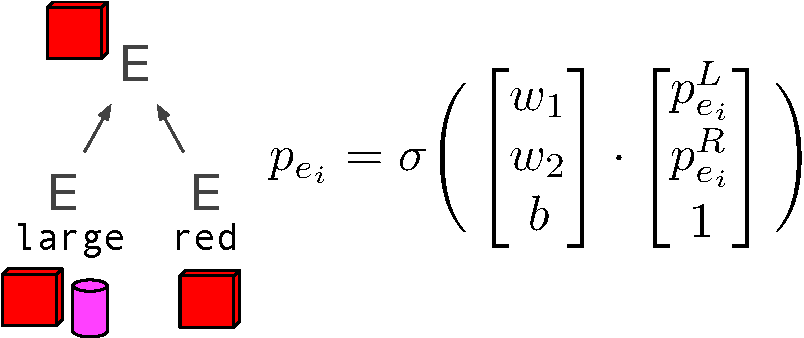
\includegraphics[width=0.5\linewidth]{chapter-4/E+E=E_new.pdf}
    \caption{\label{fig:eee} \scriptsize{\semtype{E} + \semtype{E} $\rightarrow$ \semtype{E}: This module performs a function on a pair of soft entity sets, parameterized by the model's global parameter vector $[w_{1}, w_{2}, b]$ to produce a new soft entity set. The composition function for a single entity's resulting attention value is shown. Such a composition module can be used to interpret compound nouns and entity appositions. For example, the composition module shown above learns to output the intersection of two entity sets.}}
  \end{subfigure}
  \hfill
  \begin{subfigure}[t]{.48\textwidth}
    \centering
    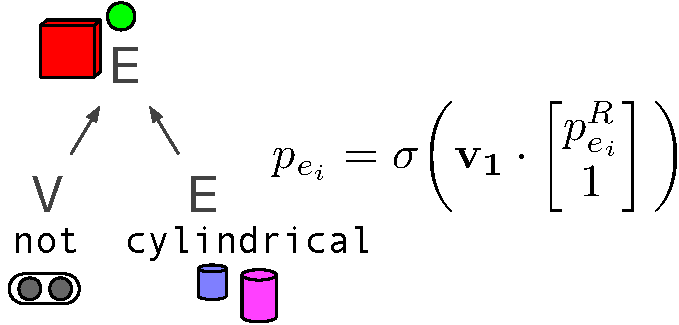
\includegraphics[width=0.5\linewidth]{chapter-4/W+E=E_new.pdf}
    \caption{\label{fig:wee}\scriptsize{\semtype{V} + \semtype{E} $\rightarrow$ \semtype{E}: This module performs a function on a soft entity set, parameterized by a word vector, to produce a new soft entity set. For example, the word \emph{not} learns to take the complement of a set of entities. The entity attention representation of the resulting span is computed by using the indicated function that takes the $v_{1} \in \mathbb{R}^{2}$ vector of the \semtype{V} constituent as a          parameter argument and the entity attention vector of the \semtype{E} constituent as a function argument.}}
  \end{subfigure}

    \smallskip

  \begin{subfigure}[t]{.48\textwidth}
    \centering
    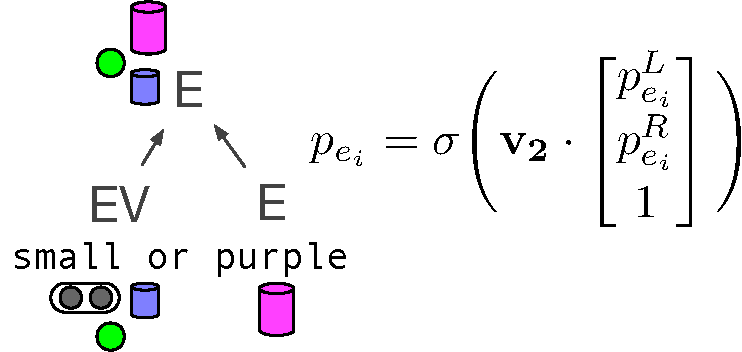
\includegraphics[width=0.6\linewidth]{chapter-4/EW+E=E_new.pdf}
    \caption{\label{fig:ewee} \scriptsize{\semtype{EV} + \semtype{E} $\rightarrow$ \semtype{E}: This module combines two soft entity sets into a third set, parameterized by the $v_{2}$ word vector. This composition function is similar to a linear threshold unit and is capable of modeling various mathematical operations such as logical conjunctions, disjunctions, differences etc. for different values of $v_{2}$. For example, the word \emph{or} learns to model set union.}}
  \end{subfigure}
  \hfill
  \begin{subfigure}[t]{.48\textwidth}
    \centering
    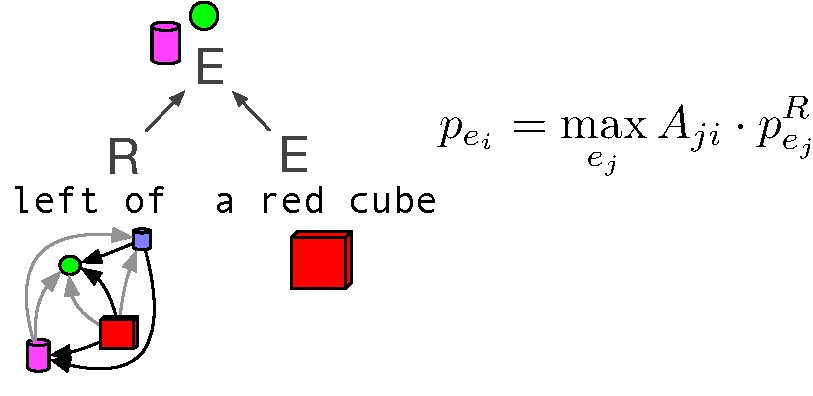
\includegraphics[width=0.6\linewidth]{chapter-4/R+E=E_new.pdf}
    \caption{\label{fig:ree}\scriptsize{\semtype{R} + \semtype{E} $\rightarrow$ \semtype{E}: This module composes a set of relations (represented as a single soft adjacency matrix) and a soft entity set to produce an output soft entity set. The composition function uses the adjacency matrix representation of the \semtype{R}-span and the soft entity set representation of the \semtype{E}-span. }}
  \end{subfigure}

   \smallskip
    % \medskip

  \begin{subfigure}[t]{.48\textwidth}
    \centering
    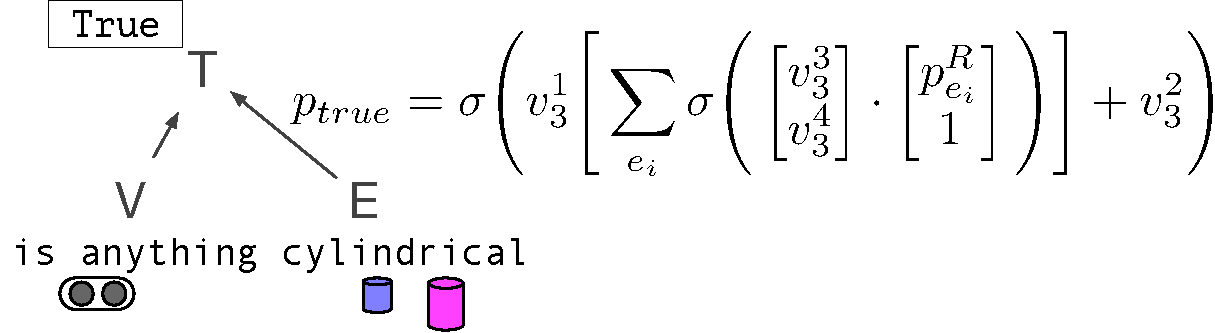
\includegraphics[width=0.85\linewidth]{chapter-4/W+E=B_new.pdf}
    \caption{\label{fig:web}\scriptsize{\semtype{V} + \semtype{E} $\rightarrow$ \semtype{T}: This module maps a soft entity set onto a soft boolean, parameterized by word vector ($v_{3}$).  The module counts whether a sufficient number of elements are in (or out) of the set. For example, the word \emph{any} should test if a set is non-empty.}}
  \end{subfigure}
  \hfill
  \begin{subfigure}[t]{.48\textwidth}
    \centering
    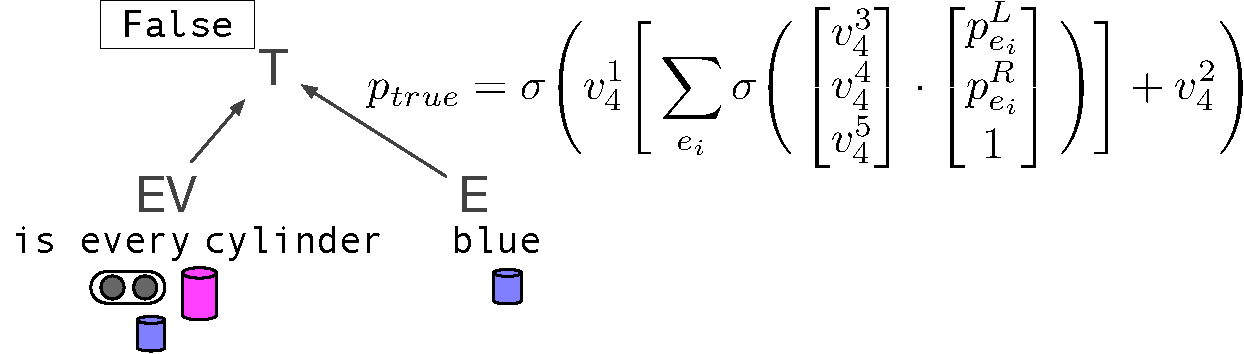
\includegraphics[width=0.85\linewidth]{chapter-4/EW+E=B_new.pdf}
    \caption{\label{fig:eweb}\scriptsize{\semtype{EV} + \semtype{E} $\rightarrow$ \semtype{T}: This module combines two soft entity sets into a soft boolean, which is useful for     modelling generalized quantifiers. For example, in \emph{is every cylinder blue}, the module can use the inner sigmoid to test if an element $e_i$ is in the set of cylinders ($p^{L}_{e_{i}}\approx 1$) but not in the set of blue things ($p^{R}_{e_{i}}\approx 0$), and then use the outer sigmoid to return a value close to 1 if the sum of elements matching this property is close to 0.  }}
  \end{subfigure}

   \smallskip
   % \medskip

  \begin{subfigure}[t]{.48\textwidth}
    \centering
    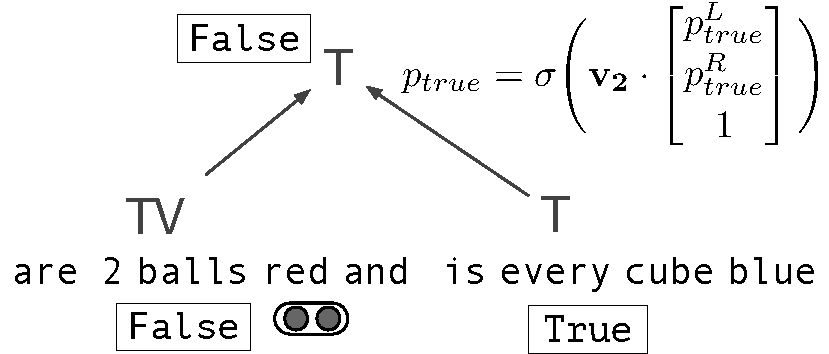
\includegraphics[width=0.6\linewidth]{chapter-4/BW+B=B_new.pdf}
    \caption{\label{fig:bwbb}\scriptsize{\semtype{TV} + \semtype{T} $\rightarrow$ \semtype{T}: This module maps a pair of soft booleans into a soft boolean using the $v_{2}$ word vector to parameterize the composition function. Similar to \semtype{EV}~+~\semtype{E}~$\rightarrow$~\semtype{E}, this module facilitates modeling a range of boolean set operations. Using the same functional form for different composition functions allows our model to use the same ungrounded word vector ($v_{2}$) for compositions that are semantically analogous.}}
  \end{subfigure}
  \hfill
  \begin{subfigure}[t]{.48\textwidth}
    \centering
    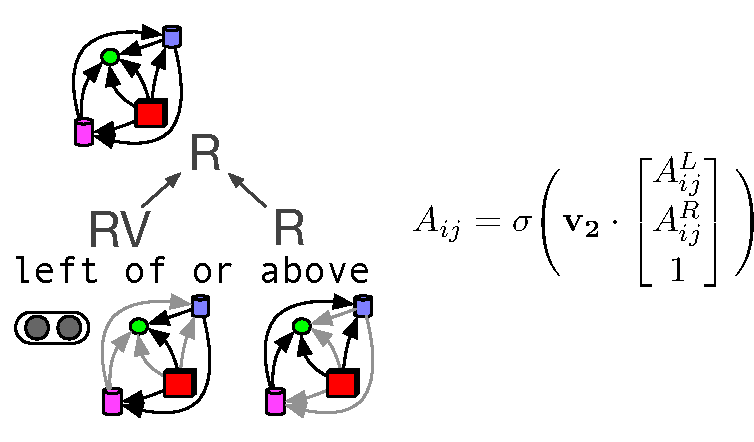
\includegraphics[width=0.6\linewidth]{chapter-4/RW+R=R_new.pdf}
    \caption{\label{fig:rwrr}\scriptsize{\semtype{RV} + \semtype{R} $\rightarrow$ \semtype{R}: This module composes a pair of soft set of relations to a produce an output soft set of relations. For example, the relations \emph{left} and \emph{above} are composed by the word \emph{or} to produce a set of relations such that entities $e_{i}$ and $e_{j}$ are related if either of the two relations exists between them. The functional form for this composition is similar to \semtype{EV}~+~\semtype{E}~$\rightarrow$~\semtype{E} and \semtype{TV}~+~\semtype{T}~$\rightarrow$~\semtype{T} modules. }}
  \end{subfigure}

  \caption{\label{fig:04-modules} \footnotesize{Composition Modules that compose two constituent span representations into the representation for the combined larger span, using the indicated equations.}}
\end{figure}
